\section{Cinemática} \label{sec:cinematica}

La cinematica es una parte de la fisica que estudia el movimiento de los sistemas mecanicos sin tomar en cuenta las fuerzas que originan dicho movimiento. Se centra en la relacion geometrica entre las articulaciones del robot y su extremo efector, de esta forma permite predecir la posicion y orientacion en funcion de las posiciones articulares, y viceversa. Comprender la cinematica es vital para entender el comportamiento del robot, hacer el control y diseño del mismo. 

\subsection{Cinemática Directa}
En el estudio de la cinemática robótica, uno de los procesos fundamentales es la cinemática directa, la cual permite determinar la posición y orientación del efector final de un robot a partir de valores conocidos de sus articulaciones. Este tipo de análisis no solo es fundamental en robótica, sino que también se aplica en otras áreas como la animación digital y el desarrollo de videojuegos. Por otro lado, el proceso inverso, conocido como cinemática inversa, consiste en calcular los valores articulares necesarios para que el efector final alcance una posición y orientación deseadas en el espacio.

Para modelar matemáticamente el movimiento de un robot con arquitectura en cadena abierta (serie), se utilizan transformaciones rígidas. Cada articulación se representa mediante una transformación [Z] que describe su movimiento relativo (rotación o traslación), mientras que cada eslabón se representa mediante una transformación [X] que define su geometría. La secuencia ordenada de estas transformaciones, desde la base hasta el efector final, permite construir el modelo cinemático completo del manipulador.

Con el fin de estandarizar este proceso, en 1955 Jacques Denavit y Richard Hartenberg propusieron una convención para la definición de estas transformaciones. Esta metodología, conocida como el método Denavit-Hartenberg (DH), establece reglas específicas para asignar sistemas de coordenadas a cada articulación y eslabón, de forma que las transformaciones entre ellos puedan representarse mediante matrices homogéneas. En esta convención, el eje z se asigna como el eje de rotación en las articulaciones rotacionales, o como el eje de traslación en las prismáticas, y todas las transformaciones se describen en términos de desplazamientos y rotaciones a lo largo o alrededor de este eje.

El método DH se ha convertido en un estándar ampliamente utilizado en robótica, gracias a su simplicidad y a la facilidad con la que puede ser implementado en entornos computacionales, permitiendo la simulación y el control preciso de manipuladores robóticos en aplicaciones tridimensionales.

\begin{figure}[H]
    \centering
    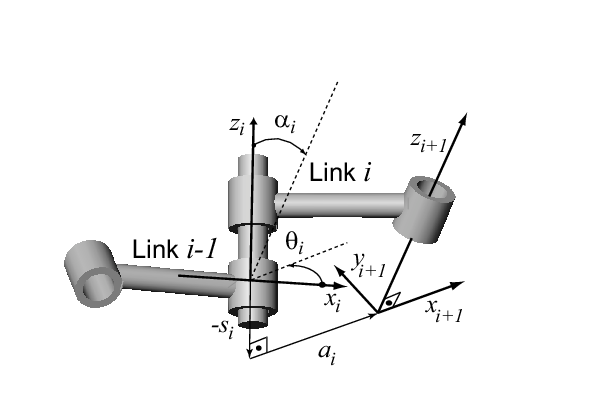
\includegraphics[width=0.75\textwidth]{matriz.png}
    \caption{DH}
    \label{fig:matriz}
\end{figure}

\subsection{Cinemática Diferencial}
La cinemática diferencial tiene como objetivo principal establecer la relación entre las velocidades de las articulaciones de un robot y la velocidad del efector final, o de cualquier otro punto asociado a su estructura. Esta relación se deriva del modelo de cinemática directa y permite obtener información clave sobre el comportamiento del robot, como la detección de singularidades, el análisis de su capacidad de maniobra y la implementación de métodos numéricos para resolver la cinemática inversa de manera iterativa, así como para controlar su movimiento dentro del espacio de trabajo.

A partir del modelo cinemático directo, representado como una función 𝑓(𝑞) que relaciona las coordenadas articulares con la posición del efector, y usando el método de Denavit-Hartenberg con matrices homogéneas, es posible construir una matriz jacobiana. En robótica, esta matriz representa la transformación entre velocidades articulares y velocidades lineales y angulares del efector final. Aunque existen distintos tipos de jacobianas, la más común es la que transforma entre el espacio articular y el espacio cartesiano.

En este modelo no se consideran fuerzas como la inercia o el rozamiento, ya que se analiza el robot como si fuera una masa puntual. Por ello, la cinemática diferencial se centra únicamente en el estudio del movimiento, sin involucrar aspectos dinámicos.

\begin{figure}[H]
    \centering
    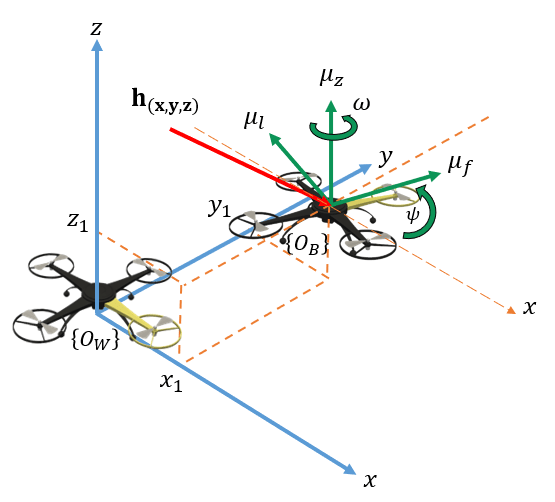
\includegraphics[width=0.50\textwidth]{img/Modelo-cinematico.png}
    \caption{Modelo diferencial}
    \label{fig:Modelo-cinematico}
\end{figure}

\subsection{Cinemática Inversa}
En robótica, la cinemática inversa se encarga de determinar los valores articulares necesarios para que el efector final del robot alcance una posición y orientación específicas. Este proceso es esencial, ya que el control del movimiento se realiza directamente sobre las articulaciones, aunque el objetivo esté en el extremo operativo.

Cuando se desea que el robot transite entre dos posturas, este procedimiento forma parte de la planificación de movimiento, donde la cinemática inversa permite convertir trayectorias deseadas en comandos concretos para los actuadores.

Este enfoque también se aplica fuera de la robótica, como en la animación digital o en simulaciones con cámaras móviles, donde se requiere ajustar articulaciones o trayectorias para lograr movimientos realistas y coherentes.

En resumen, mientras que la cinemática directa calcula la posición del efector a partir de los ángulos articulares, la cinemática inversa realiza el proceso opuesto: determina los valores de las articulaciones necesarios para alcanzar una posición deseada en el espacio.

